
\subsection{Ejercicios}
\begin{itemize}
 
\item \textbf{Ejercicio 6}  Programar un tipo de tarea TaskBatch que reciba dos parametros: total cpu y
cant bloqueos. Una tarea de este tipo debera realizar cant bloqueos llamadas bloqueantes, en
momentos elegidos pseudoaleatoriamente. En cada tal ocasion, la tarea debera permanecer
bloqueada durante exactamente un (1) ciclo de reloj. El tiempo de CPU total que utilice una
tarea TaskBatch debera ser de total cpu ciclos de reloj (incluyendo el tiempo utilizado para
lanzar las llamadas bloqueantes; no ası el tiempo en que la tarea permanezca bloqueada).

\item \textbf{Ejercicio 7} Elegir al menos dos metricas diferentes, definirlas y explicar la semantica de
su definicion. Diseñar un lote de tareas TaskBatch, todas ellas con igual uso de CPU, pero
con diversas cantidades de bloqueos. Simular este lote utilizando el algoritmo SchedRR y una
variedad apropiada de valores de quantum. Mantener fijo en un (1) ciclo de reloj el costo de
cambio de contexto y dos (2) ciclos el de migracion. Deben variar la cantidad de nucleos de
procesamiento. Para cada una de las metricas elegidas, concluir cual es el valor optimo de
quantum a los efectos de dicha metrica.

\item \textbf{Ejercicio 8} Implemente un scheduler Round-Robin que no permita la migracion de procesos
entre nucleos (SchedRR2). La asignacion de CPU se debe realizar en el momento en que se produce la carga 
de un proceso (load). El nucleo correspondiente a un nuevo proceso sera aquel
con menor cantidad de procesos activos totales (RUNNING + BLOCKED + READY). Diseñe y realice un conjunto 
de experimentos que permita evaluar comparativamente las dos implementaciones de Round-Robin.

\item \textbf{Ejercicio 9} Diseñar y llevar a cabo un experimento que permita poner a prueba la ecuanimidad 
(fairness) del algoritmo SchedLottery implementado. Tener en cuenta que, debido
al factor pseudoaleatorio involucrado, cualquier corrida puntual podrıa ser arbitrariamente
injusta; sin embargo, si se repite un mismo experimento n veces y se observan los resultados acumulativos, 
tales anomalıas deberıan ir desapareciendo conforme n aumenta. En otras
palabras, interesa mostrar en base a evidencia empırica que el algoritmo implementado efectivamente tiende 
a ser totalmente ecuanime a medida que n tiende a infinito.

\item \textbf{Ejercicio 10} Los autores del artıculo sobre lottery scheduling alegan que la optimizacion de
compensation tickets es necesaria para compensar una posible falencia del algoritmo inicial-
mente propuesto en ciertos escenarios. Diseñar y llevar a cabo un experimento apropiado para
comprobar esta afirmacion (provocar un escenario donde se manifieste el problema, comparar
simulaciones ejecutadas con y sin compensation tickets y discutir los resultados obtenidos).

\end{itemize}
\subsection{Resultados y Conclusiones}

\subsubsection[Resolución Ejercicio 6]{Ejercicio 6}

\indent Al igual que con la tarea TaskConsola, mencionaremos nuestro implementación y acontinuación de la misma 
explicaremos ciertos puntos de la misma.\\
 \begin{verbatim}
                       void TaskBatch(int pid, vector<int> params) {
                            int total_cpu = params[0];
                            int cant_bloqueos = params[1];
                            srand(time(NULL));
                            vector<bool> uso = vector<bool>(total_cpu);
                            for(int i=0;i<(int)uso.size();i++) 
                               uso[i] = false;
	                       for(int i=0;i<cant_bloqueos;i++) {
                                   int j = rand()%(uso.size());
                                   if(!uso[j])
                                      uso[j] = true;
                                   else
                                      i--; 
                                   }
                            for(int i=0;i<(int)uso.size();i++) {
                                if( uso[i] )
                                    uso_IO(pid,1); 
                                else
                                    uso_CPU(pid, 1); 
                               }
                            }
 \end{verbatim}

 \indent Para este tipo de tarea, creamos un vector de tamaño igual a $total_cpu$ el cual tendra bool, ya sea true o false
 dependiendo del uso que se le de dentro de la tarea, ya sea uso\_IO o uso\_CPU. En caso de ser uso\_IO sera true, y sino false.\\
 Luego, utilizaremos un ciclo que ira desde 0 hasta el tamaño del vector y dependiendo el valor booleano, usará la funciones
 dadas por la catedra uso\_IO o uso\_CPU.\\
 
 \subsubsection[Resolución Ejercicio 7]{Ejercicio 7}
 Las métricas elegidas fueron:
\begin{itemize}
 \item \textbf{Turnaround}: Es el intervalo de tiempo desde que un proceso es cargado hasta que este finaliza su ejecución.
 \item \textbf{Waiting Time}: Es la suma de los intervalos de tiempo que un proceso estuvo en la cola de procesos $ready$.
\end{itemize}

\indent \indent Como las tareas TaskBatch se bloquean pseudoaleatoriamente, 
para obtener datos relevantes tomamos un promedio de las mediciones.\\
\indent A la hora de encarar la experimentación, lo que realizamos fue simular corridas con 
varios quantum para poder obtener una aproximación del efecto del $quantum$ en la ejecución del lote de tareas. 

\indent De esta aproximación, se confeccionaron gráficos de turnaround time en función del quantum, 
referente al estudio con 2 y 3 núcleos, los cuales se proveerán a continuación:\\

\indent Luego de realizar mediciones con distintos $quantum$, tomamos la decisión de trabajar con los mismos $quantum$ para cada nucleo
al trabajar con más de 1 core. (Se muestra acontinuación un gráfico para demostrar que no era una decisión acertada trabajar
con disversos $quantum$ para cada core).

\begin{center}
    	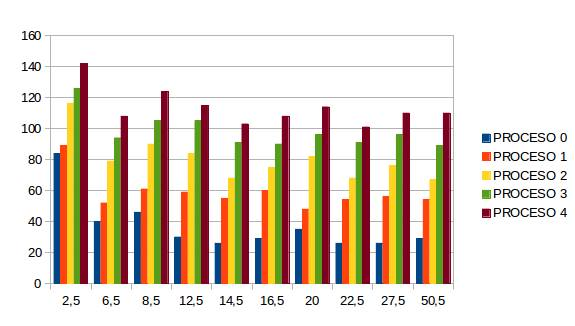
\includegraphics[width=1\textwidth]{./EJ7/turnarounddistquan.png}
	{Turnaround - 2 core - Prueba Quantum distintos por Core}\\
	{$Eje X = Quantum; $\\$ Eje Y = Tiempo$}\\
 \end{center}

\indent Al realizar, este gráfico y varias mediciones con distintos $quantum$ por core, nos dimos cuenta que no terminaban
siendo mediciones rigurosas, ya que una tarea podia estar corriendo con distintos tiempos por la migracion de procesos por core.\\
\indent Por ende, optamos por realizar mediciones con igualdad de $quantum$ por core para obtener la mejor performance posible.\\
 
 \indent Por consiguiente, al trabajar con las nuevas mediciones, conjeturamos las siguientes hipótesis:
 
 \begin{itemize}
  \item Con 2 nucleos las mediciones de tiempo tienden a estabilizarse a partir de un $quantum$ igual a 9.
  \item Con 3 nucleos las mediciones de tiempo tienden a estabilizarse a partir de un $quantum$ igual a 11.
 \end{itemize}
 \begin{center}
 \textbf{Turnaround Time} 
  \end{center}

 \begin{center}
 \textbf{2 Core}
 \end{center}
  A continuación se muestran los Diagramas de Gantt más relevantes:
  
  \begin{center}
    	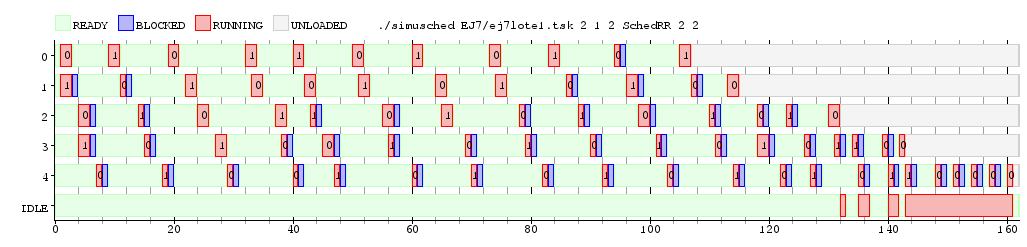
\includegraphics[width=450pt]{./EJ7/ej7tour2core1quan.png}
	{$Lote 1$ - Turnaround - 2 core - Quantum igual a 2}	
 \end{center}

   \begin{center}
    	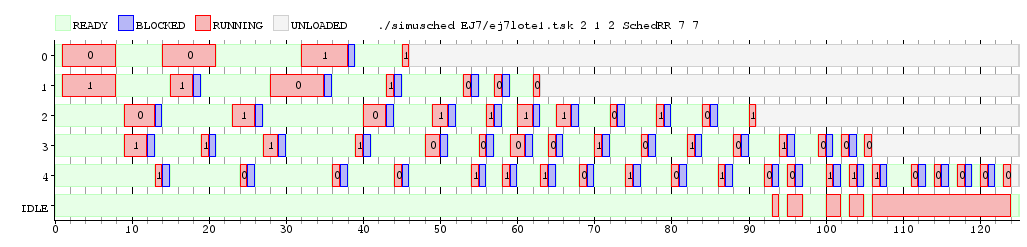
\includegraphics[width=450pt]{./EJ7/ej7tour2core3quan.png}
	{$Lote 1$ - Turnaround - 2 core - Quantum igual a 7}	
 \end{center}
 
 
 \indent La performance empieza a mejorar a medida que el $quantum$ aumenta.
 
   \begin{center}
    	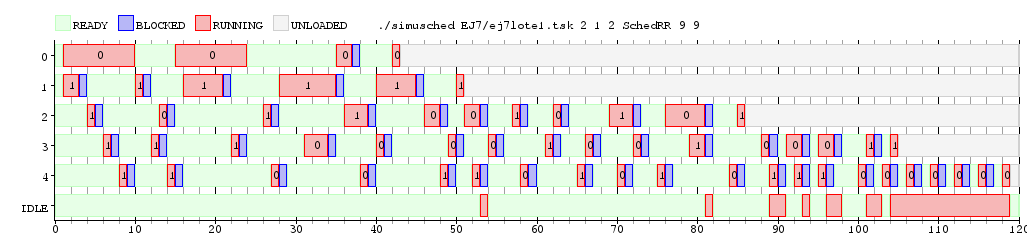
\includegraphics[width=450pt]{./EJ7/ej7tour2core4quan.png}
	{$Lote 1$ - Turnaround - 2 core - Quantum igual a 9}	
 \end{center}

  
   \indent La performance sigue mejorando,a partir de este valor, el desempeño comienza a estabilizarse, como muestran los siguiente dos gráficos. 
   Las pequeñas diferencias en los valores responden a la pseudoaleatoridad de las tareas TaskBatch.\\
  
   \begin{center}
    	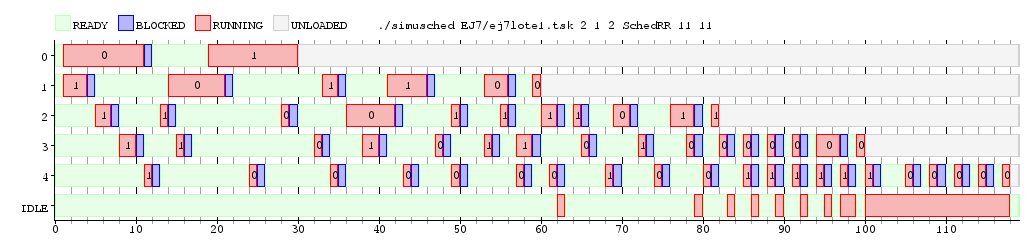
\includegraphics[width=450pt]{./EJ7/ej7tour2core5quan.png}
	{$Lote 1$ - Turnaround - 2 core - Quantum igual a 11}	
 \end{center}
 

    \begin{center}
    	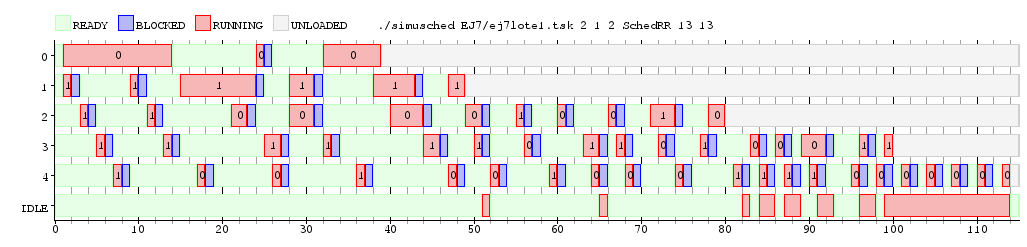
\includegraphics[width=450pt]{./EJ7/ej7tour2core8quan.png}
	{$Lote 1$ - Turnaround - 2 core - Quantum igual a 13}	
 \end{center}

 \indent Como mencionamos, las mediciones tienden a estabilizarse con un $quantum$ igual a 9, pero la mejor performance
 obtenida es con un $quantum$ igual a 13, teniendo en cuenta la pseudoaleatoridad del tipo de tarea utilizada.
 \indent Se puede observar en la primer figura que a pesar de trabajar con 2 cores, al tener un quantum bajo (igual a 2) 
 el costo es alto.\\
  
  
 \begin{center}
    	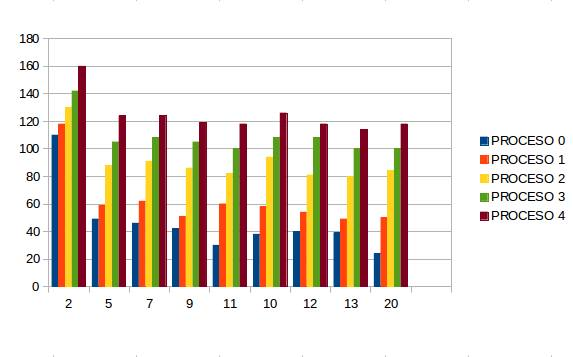
\includegraphics[width=1\textwidth]{./EJ7/tour2core.png}
	{Turnaround - 2 core}	\\
	{$Eje X = Quantum$\\$ Eje Y = Tiempo$}\\
 \end{center} 
 
 \begin{center}
  \textbf{Waiting Time}
 \end{center}

  \begin{center}
    	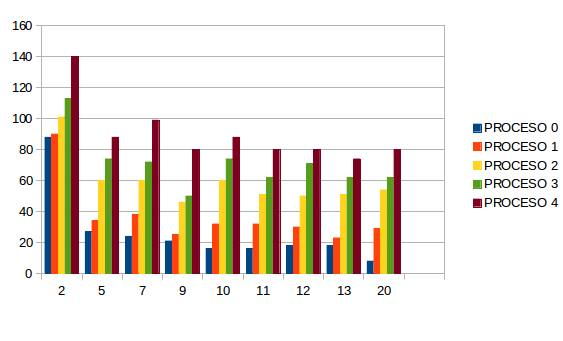
\includegraphics[width=1\textwidth]{./EJ7/waiting2core.jpg}
	{Waiting Time - 2 core}	\\
	{$Eje X = Quantum$\\$Eje Y = Tiempo$}\\
 \end{center} 
 
 \indent Con este tipo de metrica, se comienza a estabilizar a partir del $quantum$ igual a 5, obteniendo su mejor
 performance con el $quantum$ igual a 13.\\
 
   \begin{center}
   \textbf{3 Core}
   \end{center}
   \indent A continuación, al igual que con 2 cores, mostraremos los Diagramas de Gantt mas relevantes:
   
   \begin{center}
    	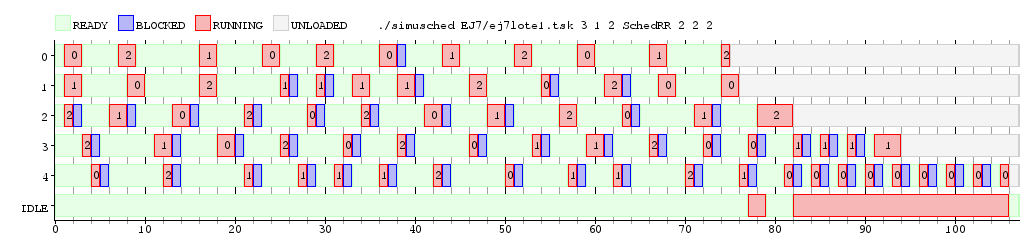
\includegraphics[width=450pt]{./EJ7/ej7tour3core1quan.png}
	{$Lote 1$ - Turnaround - 3 core - Quantum igual a 2}	
 \end{center}

 \indent Se observa que al tener otro core mas,a diferencia de con 2, a pesar de estar con un $quantum$ bajo,
 la performance mejora bastante.\\ 
 
   \begin{center}
    	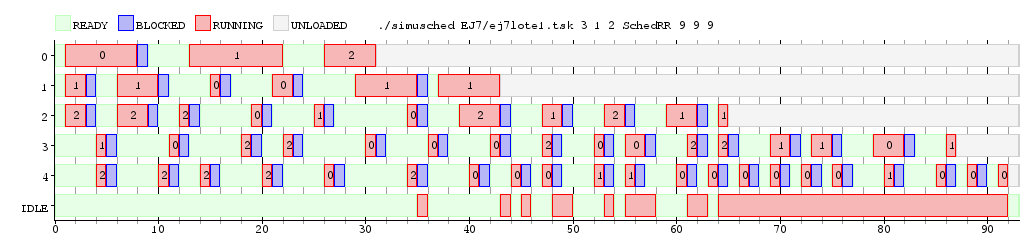
\includegraphics[width=450pt]{./EJ7/ej7tour3core4quan.png}
	{$Lote 1$ - Turnaround - 3 core - Quantum igual a 9}	
 \end{center}
 
 
 \indent La performance empieza a mejorar a medida que el $quantum$ aumenta.
 
   \begin{center}
    	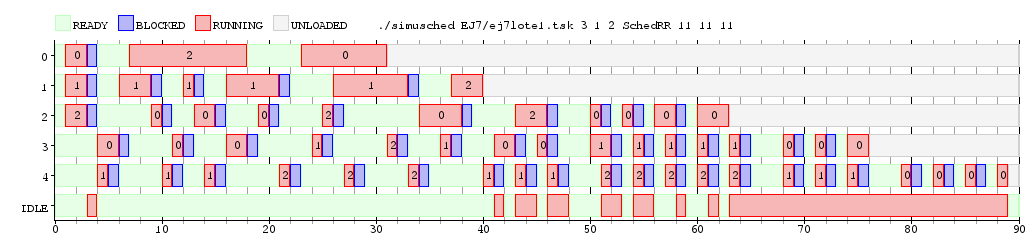
\includegraphics[width=450pt]{./EJ7/ej7tour3core5quan.png}
	{$Lote 1$ - Turnaround - 3 core - Quantum igual a 11}	
 \end{center}
  
   \begin{center}
    	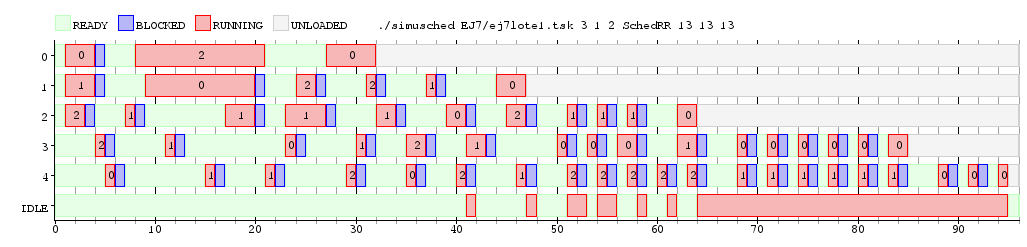
\includegraphics[width=450pt]{./EJ7/ej7tour7core6quan.png}
	{$Lote 1$ - Turnaround - 3 core - Quantum igual a 13}	
 \end{center}
 
 \begin{center}
    	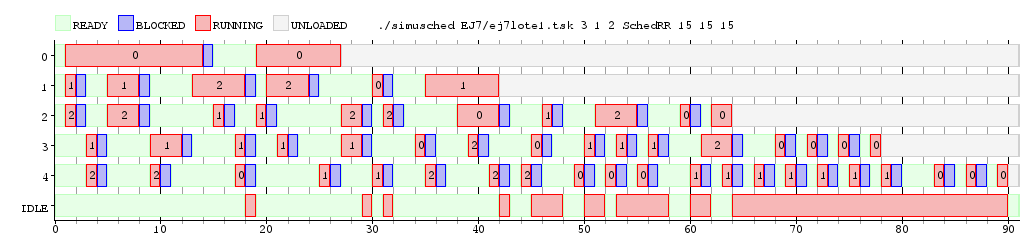
\includegraphics[width=450pt]{./EJ7/ej7tour8core6quan.png}
	{$Lote 1$ - Turnaround - 3 core - Quantum igual a 15}	
 \end{center}
 
 \indent A diferencia que en nuestra hipótesis conjeturada para con dos cores, con un $quantum$ igual a 11 se obtiene la mejor
 performance, pero teniendo en cuenta la pseudoaleatoridad del tipo de tarea con la que se trabajo, a partir del $quantum$ igual
 a 9 ya se estabiliza notoriamente.\\
   
    \begin{center}
    	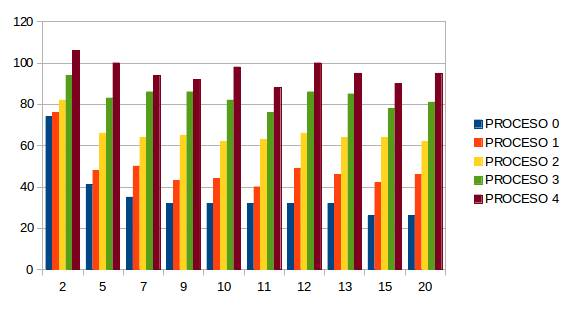
\includegraphics[width=1\textwidth]{./EJ7/tour3core.png}
	{Turnaround - 3 core}\\
	{$Eje X = Quantum $\\$ Eje Y = Tiempo$}\\
 \end{center} 
  
   \begin{center}
  \textbf{Waiting Time}
 \end{center}

  \begin{center}
    	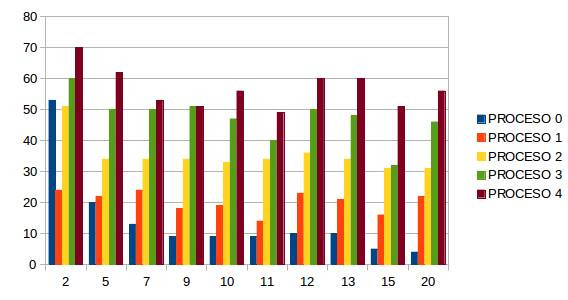
\includegraphics[width=1\textwidth]{./EJ7/waintin3core.jpg}
	{Waiting Time - 3 core}	\\
	{$Eje X = Quantum $\\$Eje Y = Tiempo$}\\
 \end{center} 
 
   \indent Con este tipo de metrica,se obteniene a diferencia de con Turnaround  su mejor
   performance con el $quantum$ igual a 15.\\
  
 \begin{center}
  \textbf{Conclusiones}
 \end{center}


\indent \indent La diferencia entre los valores de quantum entre los casos se puede atribuir a que cada vez que 
agregamos un núcleo aumentamos la posibilidad de una migración de la tareas.\\
\indent \indent En todos lo casos se observa la influencia negativa que proviene de elegir un quantum con valores pequeños.\\
\indent \indent Agregar núcleos de procesamiento mejora significativamente la performance de acuerdo a la métricas con las que
trabajamos, al permitir más procesamiento en pararelo y disminuyendo los waiting time de las tareas.\\
\indent \indent  Fijada una cantidad de núcleos, aumentar el valor del quantum también mejora la performance, 
especialmente los tiempos referidos a las tareas que menos cantidad de bloqueos tienen. 
Igualmente, a partir de cierto valor de quantum, las mejoras en la performance dejan de ser muy significativas. 
Esto se produce a que las tareas con mas cantidad de bloqueos en algun momento dejan de consumir todo
su quantum si seguimos aumentando el valor. 
 
 
 
\subsubsection[Resolución Ejercicio 8]{Ejercicio 8}
\indent \indent La idea central de esta version de Round-Robin es que no permita migración entre núcleos y esto se basa en utilizar una cola FIFO por cada núcleo, donde se encolarán aquellas tareas a las que se asignó el core correspondiente. \\ 
\indent Para implementar este algoritmo, el Round-Robin 2, utilizamos varias estructuras. Estas son:\\
\begin{itemize}
\item Los vectores $quantum$ y $quantumActual$, que cumplen la misma función que en nuestra implementación de Round-Robin.\\
\item El vector de colas $colas$, donde en la posición $i$ se encontrará la cola de tareas correspondiente a ese núcleo de procesamiento.\\
\item El diccionario $bloqueados$, donde mantenemos aquellas tareas que se bloquearon con su número de core correspondiente y que nos permitirá, cuando la tarea se desbloquee, reubicarla en la cola del core que le corresponde.\\ 
\item El vector de enteros $cantidad$, cuya única función será tener en la posición $i$ la cantidad de tareas bloqueadas, activas o en estado ready que están asignadas al core $i$ y que nos servirá para determinar a qué núcleo se asignará una tarea al momento de cargarla.\\
\end{itemize}

\indent \indent Cuando se carga una tarea, se chequea cuál es el core que menor cantidad de procesos activos totales tiene asignados(haciendo uso de la posición respectiva del vector $cantidad$). Una vez que se obtiene dicho núcleo, se agrega la tarea a la cola de tareas correspondiente al core y se actualiza la cantidad de tareas activas para ese núcleo sumándole uno.\\
\indent \indent Al bloquearse una tarea, se define una entrada en el diccionario $bloqueados$ con el pid y el núcleo correspondiente. De esta manera, al desbloquearse, obtenemos el core en el que debe correr, eliminamos la entrada del diccionario y encolamos nuevamente el pid a la cola del núcleo en cuestión. De esta manera resolvemos parcialmente el problema de no permitir la migración entre cores.\\
\indent \indent Finalmente, cuando una tarea termina, se actualiza la cantidad correspondiente al núcleo restándole uno. Solamente a la hora de cargar la tarea y cuando una tarea termina se modifica dicha variable. De esta manera, aunque una tarea se bloquee seguirá reflejada en la cantidad del núcleo, lo que nos permitirá seguir el criterio que nos pidieron en la consigna a la hora de asignarle un core a la tarea.\\

\indent \indent Como esta modificación de Round-Robin no permite migración entre cores, 
conjeturamos ciertos puntos:\\
\begin{itemize}
 \item Dados un mismo lote de tareas y una misma configuración del scheduler (tick de costo en cambio de contexto y quantum)
 un único núcleo de procesamiento,  ambos algoritmos deben comportarse de la misma manera. 
  \item Comportamiento más eficiente en el Round-Robin 2 en lotes de tareas que se bloquean una gran cantidad de veces, o  en configuraciones con $quantums$ pequeños. 
  Esto surge de que dichos escenarioshacen más proclive al Round-Robin a impulsar más cambios de contexto, 
  con la posible penalidad de darse un cambio de núcleo, algo que puede ser muy costoso.
  \item El Round Robin debería comportarse más eficientemente en situaciones en las cuales el Round-Robin 2 pierde la posibilidad de parelelismo. 
  Por ejemplo, varias tareas quedaron asignadas a un núcleo mientras los demás están libres. Generando que varios nucleos queden ociosamente bastante tiempo.
  
 \end{itemize}

 \indent A continuación, mostraremos los experimentos diseñados para demostrar y explicar un poco mejor lo conjeturado:
 
 \indent Arrancando con nuestra primer conjetura:
 
 \begin{center}
  \textbf{Dados un mismo lote de tareas y una misma configuración del scheduler con un único núcleo de procesamiento, 
 ambos algoritmos deben comportarse de la misma manera. }
 \end{center}

 
 \indent Trabajando con el siguiente lote:
 
 \begin{verbatim}
                                     TaskCPU 70
                                     TaskConsola 2 4 5
                                     TaskCPU 40
                                     TaskConsola 3 2 3
                                     TaskCPU 30
 \end{verbatim}

  \begin{center}
    	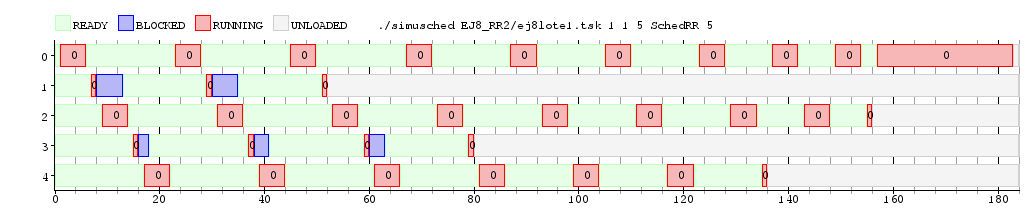
\includegraphics[width=450pt]{./EJ8_RR2/dif1corerr.png}
	{$Lote 1$ - Round Robin - 1 core - Quantum = 5 - cambio de contexto = 1}	
 \end{center}
 
 \begin{center}
    	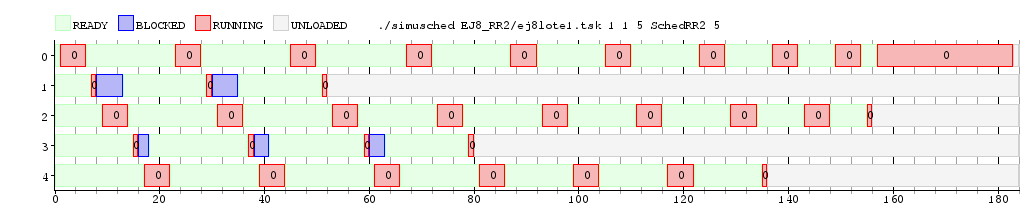
\includegraphics[width=450pt]{./EJ8_RR2/dif1corerr2.png}
	{$Lote 1$ - Round Robin 2 - 1 core - Quantum = 5 - cambio de contexto = 1}	
 \end{center}
 
 \indent Se ve a simple vista, la igualdad entre ambos con este tipo de lote.\\
 
 \indent Ahora, con un lote distinto:
 
 \begin{verbatim}
                                     TaskCPU 70
                                     TaskConsola 5 6 7
                                     TaskCPU 40
                                     TaskConsola 10 9 8
                                     TaskCPU 30
 \end{verbatim}
 
   \begin{center}
    	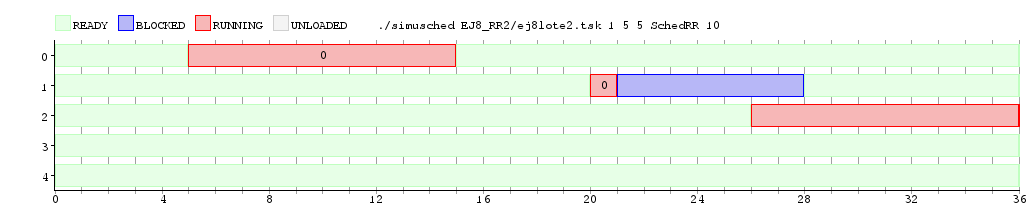
\includegraphics[width=450pt]{./EJ8_RR2/dif2corerr.png}
	{$Lote 2$ - Round Robin - 1 core - Quantum = 10 - cambio de contexto = 5}	
 \end{center}
 
 \begin{center}
    	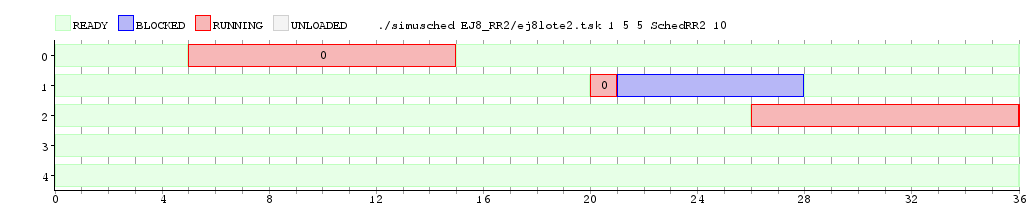
\includegraphics[width=450pt]{./EJ8_RR2/dif2corerr2.png}
	{$Lote 2$ - Round Robin 2 - 1 core - Quantum = 10 - cambio de contexto = 5}	
 \end{center}
 
 \indent Nuevamente, observamos la misma igualdad entre ambos. De la unica manera en la cual se podria producir un cambio
 entre ambos Diagramas es alterando el cambio de contexto para uno y no para el otro.
 
 \begin{center}
    	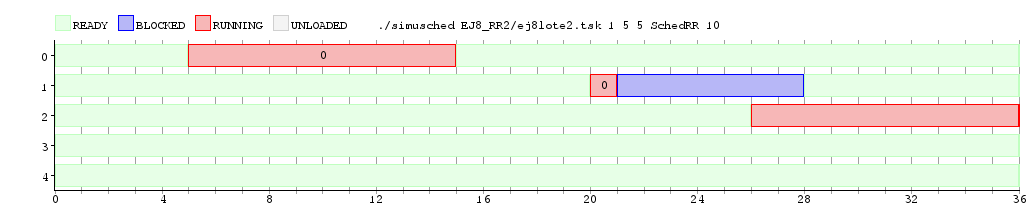
\includegraphics[width=450pt]{./EJ8_RR2/dif3corerr.png}
	{$Lote 2$ - Round Robin - 1 core - Quantum = 10 - cambio de contexto = 5}	
 \end{center}
 
 \begin{center}
    	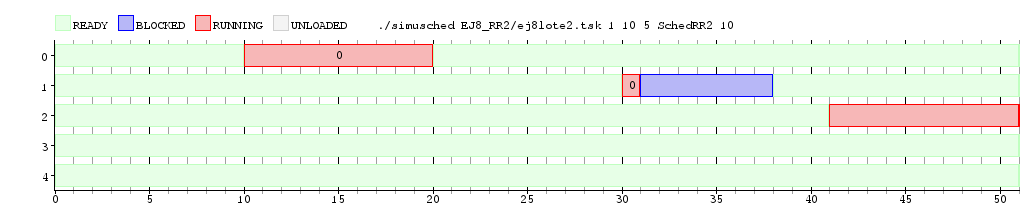
\includegraphics[width=450pt]{./EJ8_RR2/dif3corerr2.png}
	{$Lote 2$ - Round Robin 2 - 1 core - Quantum = 10 - cambio de contexto = 10}	
 \end{center}
 
  \indent Aqui se ve las diferencias como lo mencionamos, por ende, podemos concluir que como el Round Robin 2 solo fue modificado 
  para tener colas independientes para cada nucleo, al trabajar con 1 solo core, no se veran diferencias.\\

  \indent Continuamos con la siguiente conjetura realizada:
  
  \begin{center}
   \textbf{Comportamiento más eficiente en el Round-Robin 2 en lotes de tareas que se bloquean una gran cantidad de veces, 
   o  en configuraciones con $quantums$ pequeños.}
  \end{center}
  
  \indent Arrancaremos mostrando casos con cambios de contexto y quantum pequeños:
  
   \begin{center}
    	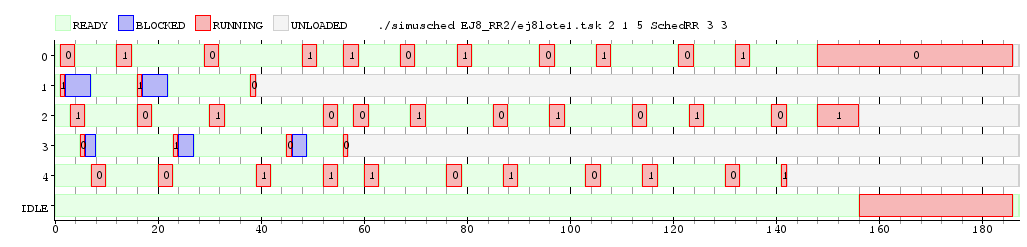
\includegraphics[width=450pt]{./EJ8_RR2/dif4corerr.png}
	{$Lote 1$ - Round Robin - 2 core - Quantum = 3 - cambio de contexto = 1}	
 \end{center}
 
 \begin{center}
    	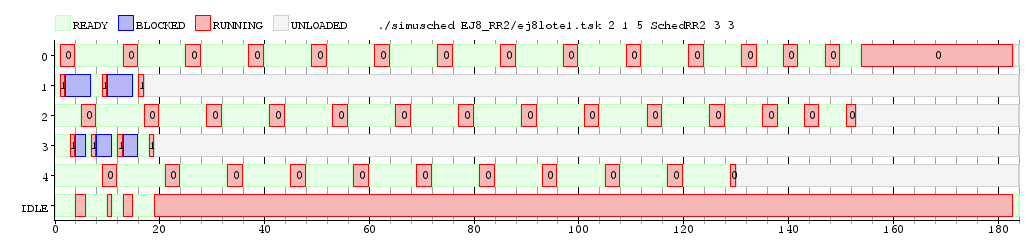
\includegraphics[width=450pt]{./EJ8_RR2/dif4corerr2.png}
	{$Lote 1$ - Round Robin 2 - 2 core - Quantum = 3 - cambio de contexto = 1}	
 \end{center}
 
 
\indent Se puede observar, una mejoria leve del Round Robin 2. Con la modificación realizada en el Round Robin 2,
no habria ninguna modificacion en caso de aumentar o disminuir el cambio de migracion ya que este no lo permite.\\

\indent Ahora, si trabajamos con tareas que utilicen el CPU y se bloqueen mucho mas podremos notar la mejor performance
de este nuevo scheduler.\\

\begin{verbatim}
                                     TaskCPU 40
                                     TaskBatch 10  5
                                     TaskCPU 50
                                     TaskBatch 15 8
                                     TaskCPU 10

\end{verbatim}


   \begin{center}
    	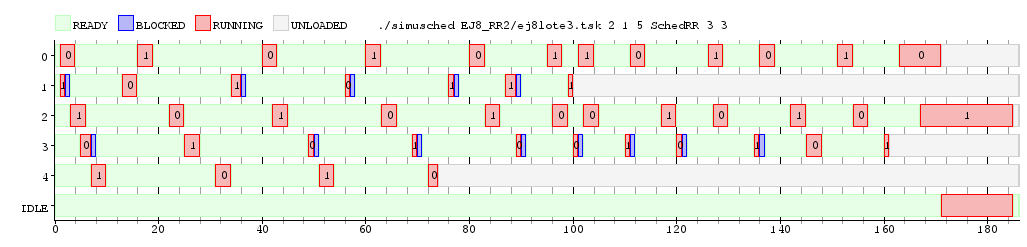
\includegraphics[width=450pt]{./EJ8_RR2/dif5corerr.png}
	{$Lote 3$ - Round Robin - 2 core - Quantum = 3 - cambio de contexto = 1}	
 \end{center}
 
 \begin{center}
    	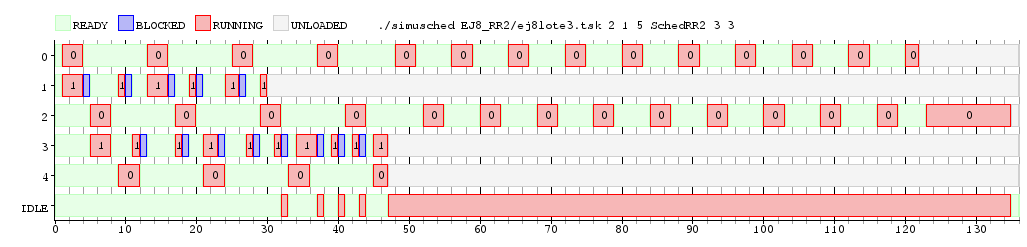
\includegraphics[width=450pt]{./EJ8_RR2/dif5corerr2.png}
	{$Lote 3$ - Round Robin 2 - 2 core - Quantum = 3 - cambio de contexto = 1}	
 \end{center}

 \indent Se ve a simple vista, como el RR2 es mucho mejor, y termina aprox 50 milisegundos antes.\\
 Como mencionamos anteriormente, si el cambio de migracion se alterase no tendria incidencia para este RR2 ya que 
 no admite migracion de tareas, mientras que el anterior scheduler si, pudiendo empeorar a su vez su performance en caso
 de que el coso fuese mayor.\\
 
 \indent Por consiguiente, podemos afirmar, que nuestro RR2 sera notablemente mejor con tareas que utilicen el CPU y se bloqueen
 bastante tiempo.\\
 
 \indent Por ulimto, demostraremos nuestra ultima conjetura: 
 
  \begin{center}
   \textbf{El Round Robin debería comportarse más eficientemente en situaciones en
   las cuales el Round-Robin 2 pierde la posibilidad de parelelismo.}
  \end{center}
  
  \indent Para probar esta conjetura, utilizamos tareas que demanden mas al CPU como $TaskCPU$.\\
  
\begin{verbatim}
                                     TaskCPU 40
                                     TaskCPU 15
                                     TaskCPU 50
                                     TaskCPU 30
                                     TaskCPU 50
\end{verbatim}

\begin{center}
    	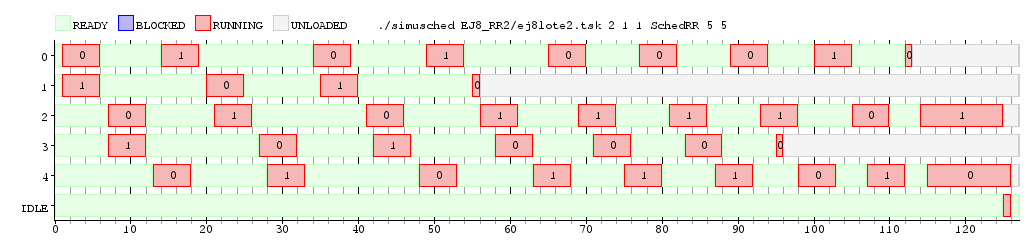
\includegraphics[width=450pt]{./EJ8_RR2/dif10corerr.png}
	{$Lote 3$ - Round Robin - 2 core - Quantum = 5 - cambio de contexto = 1}	
 \end{center}
 
 \begin{center}
    	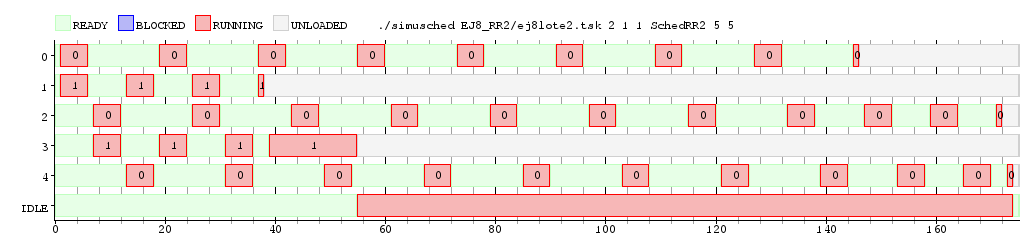
\includegraphics[width=450pt]{./EJ8_RR2/dif10corerr2.png}
	{$Lote 3$ - Round Robin 2 - 2 core - Quantum = 5 - cambio de contexto = 1}	
 \end{center}

 \indent Es notorio en estos gráficos cómo el Round-Robin, responde mejor que el Round-Robin 2. 
 Esto es porque puede trabajar con procesamiento en paralelo, mientras que el Round-Robin 2 no, 
 porque las 3 tareas quedaron asignadas a un core (el numero 0), aunque haya un core ocioso por un largo tiempo.\\
 En este caso, pagando el costo de migración se obtiene una mejor performance.\\

\indent Con estos experimentos realizados logramos observar los comportamientos que habíamos conjeturado concluyendo que son
ciertos. 

\indent Por ende, podemos concluir que el Round-Robin 2 responde de manera positiva para lotes con tareas de gran cantidad de bloqueos
y de manera negativa al no poder paralelizar ciertos procesos.\\
  
\subsubsection[Resolución Ejercicio 9]{Ejercicio 9}

\subsubsection[Resolución Ejercicio 10]{Ejercicio 10}

\indent Hemos encontrado, luego de varios experimentos, que este tipo de scheduler presenta graves problemas cuando 
se tienen varias tareas con mismo deadline.\\
Al no presentar ningun tipo de especificación, este scheduler, al no saber cuanto durará la tarea ejecuta cualquiera sin
darle prioridad al orden de los deadline dado en el lote de tarea.\\
A continuación, expondremos un caso practico donde se puede ver como impacta dentro del desempeño del scheduler el orden en el que son
cargadas las tareas pero la falta de informacion del scheduler imposibilita la posibilidad de cumplir la propiedad
de carga respetando los deadline dados.\\

Uno de los lotes propuestos, fue el siguiente:\\
\\\\\\\\
\begin{verbatim}
                                         $5:
                                         TaskCPU 40
                                         $25:
                                         TaskConsola 2 5 8
                                         $25:
                                         TaskCPU 100
                                         $25:
                                         TaskConsola 1 1 5

\end{verbatim}

Donde el resultado que obtuvimos fue el siguiente:\\

 \begin{center}
    	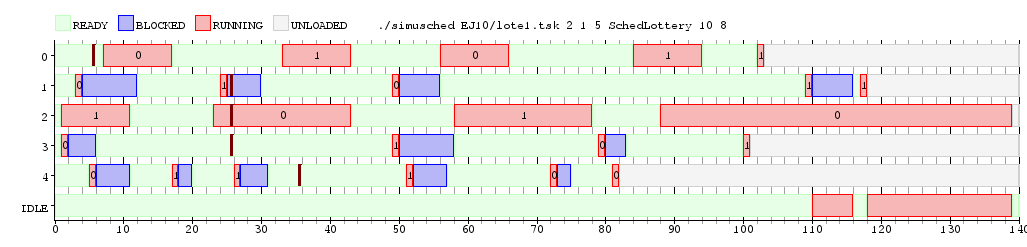
\includegraphics[width=450pt]{./ej10p7con.png}
	{$Lote 2$ - Lottery - 2 core}	
 \end{center}

\indent Como se puede observar, tanto el proceso 2 como 3 y 4 presentan el mismo deadline y terminan corriendo
fuera del orden acordado a pesar de estar trabajando con varios cores a la ves.\\

\indent Tambien, desarrollamos experimentos para los casos en que los deadline no sean los mismos, y obtuvimos
resultados similares.\\
Uno de los lotes fue el siguiente:

\begin{verbatim}
                                         $5:
                                         TaskCPU 40
                                         $25:
                                         TaskConsola 2 5 8
                                         $30:
                                         TaskCPU 100
                                         $35:
                                         TaskConsola 1 1 5

\end{verbatim}

Donde el resultado fue:\\

 \begin{center}
    	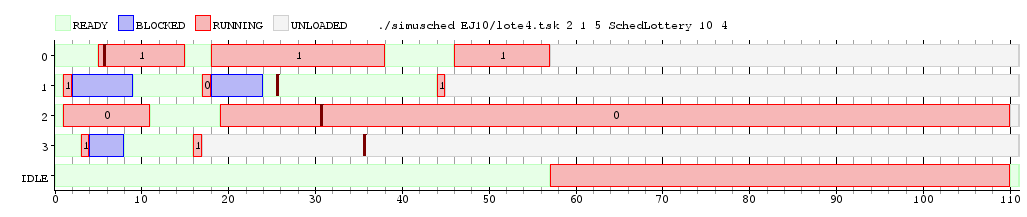
\includegraphics[width=450pt]{./ej10p12con.png}
	{$Lote 4$ - Lottery - 2 core}	
 \end{center}

 \indent Como vemos, a pesar de tener distintos valores de deadline no se respeta el orden en este scheduler.\\
